% Stylised redrawing of Diederichs et al., Phys. Rev. Lett. 135, 015001
% (2025), Fig. 2(b). Horizontal and vertical witness emittances along the
% propagation coordinate, parametrised by the dimensionless detuning
% Delta/g between the two transverse betatron frequencies. Curves follow
% the Rabi-exchange structure of the m=2 mixing loop rather than the
% specific nonlinearity coefficients of the original simulation.
%
% Build:  pdflatex diederichs_mixing.tex
\documentclass[tikz,border=4pt]{standalone}
\usepackage{amsmath}
\usepackage{amssymb}
\usepackage{pgfplots}
\pgfplotsset{compat=1.18}
\usetikzlibrary{arrows.meta}

\definecolor{onres}{RGB}{198, 60,  50}       % loop closed (full exchange)
\definecolor{partres}{RGB}{210, 130, 40}     % partial resonance (orange)
\definecolor{offres}{RGB}{60,  110, 160}     % loop broken (preserved)

\begin{document}
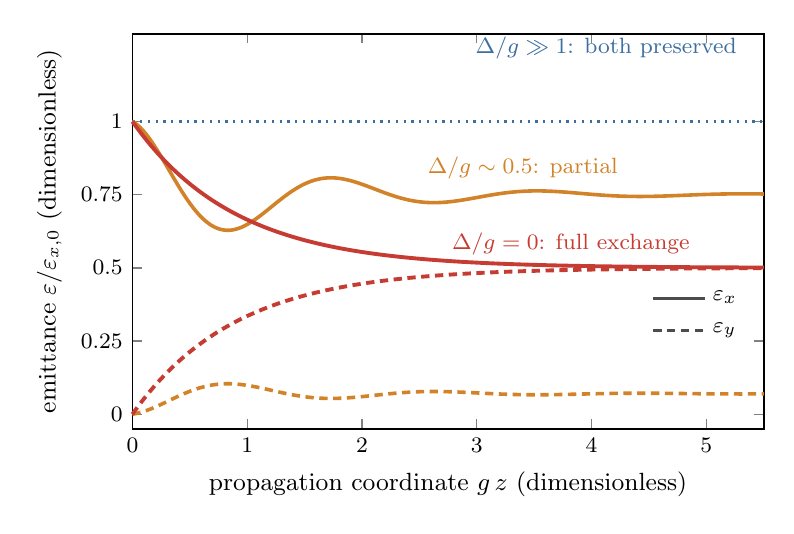
\begin{tikzpicture}

  \begin{axis}[
      width=9.6cm, height=6.6cm,
      xlabel={propagation coordinate $g\,z$ (dimensionless)},
      ylabel={emittance $\varepsilon / \varepsilon_{x,0}$ (dimensionless)},
      xmin=0, xmax=5.5,
      ymin=-0.05, ymax=1.30,
      xtick={0,1,2,3,4,5},
      ytick={0, 0.25, 0.5, 0.75, 1.0},
      tick align=inside,
      major tick length=0.12cm,
      tick style={line width=0.5pt},
      axis line style={line width=0.6pt},
      label style={font=\small},
      tick label style={font=\footnotesize},
      enlargelimits=false,
      clip=false,
  ]

    % ----- Reference: "preserved" baseline for Delta/g >> 1 (both emittances
    % stay at their initial values; rendered as a thin dotted line distinct
    % from the exchange curves' solid/dashed convention).
    \addplot[offres, line width=0.8pt, dotted, domain=0:5.5, samples=40]
      {1.0};
    \node[font=\footnotesize, color=offres, anchor=south east] at
      (axis cs:5.35, 1.18) {$\Delta/g \gg 1$: both preserved};

    % ----- Partial resonance (Delta/g ~ 0.5): incomplete exchange with a
    % visible oscillation from the partially-resonant sub-population.
    % This is the scientifically non-trivial panel of Diederichs Fig. 2(b).
    \addplot[partres, line width=1.3pt, domain=0:5.5, samples=260]
      {0.75 + 0.25 * exp(-x/1.2) * cos(deg(3.5*x))};             % eps_x (partial)
    \addplot[partres, line width=1.3pt, densely dashed, domain=0:5.5, samples=260]
      {0.07 - 0.07 * exp(-x/1.2) * cos(deg(3.5*x))};             % eps_y (partial)

    % ----- On-resonance (Delta/g = 0): full exchange, m=2 loop active.
    \addplot[onres, line width=1.4pt, domain=0:5.5, samples=200]
      {0.5 + 0.5 * exp(-x/0.9)};                                 % eps_x: 1 -> 0.5
    \addplot[onres, line width=1.4pt, densely dashed, domain=0:5.5, samples=200]
      {0.5 - 0.5 * exp(-x/0.9)};                                 % eps_y: 0 -> 0.5

    % ----- Inline per-curve labels.
    \node[font=\footnotesize, color=partres, anchor=south] at
      (axis cs:3.4, 0.77) {$\Delta/g \sim 0.5$: partial};
    \node[font=\footnotesize, color=onres, anchor=west] at
      (axis cs:2.7, 0.58) {$\Delta/g = 0$: full exchange};

    % ----- Small solid/dashed key in the low-y region where it doesn't conflict.
    \node[font=\footnotesize, anchor=south east] at (axis cs:5.35, 0.22)
      {\begin{tabular}{@{}r@{\;}l@{}}
        \tikz{\draw[line width=1.3pt, black!70] (0,0)--(0.45,0);} & $\varepsilon_x$ \\[2pt]
        \tikz{\draw[line width=1.1pt, black!70, densely dashed] (0,0)--(0.45,0);} & $\varepsilon_y$
      \end{tabular}};

  \end{axis}

\end{tikzpicture}
\end{document}
